\documentclass[12pt,a4paper]{article}
\usepackage[utf8]{inputenc}
\usepackage[OT1]{fontenc}
\usepackage{amsmath}
\usepackage{amsfonts}
\usepackage{amssymb}
\usepackage{graphicx}
\usepackage{tikz}
\usepackage{pgfplotstable}
\usepackage{mathtext}

\usepackage[T1]{fontenc}
\usepackage[utf8]{inputenc}
\usepackage[english, bulgarian, russian]{babel}

\usepackage{tikz}
\usepackage{pgfplots}
\usepackage{indentfirst}
\usepackage[export]{adjustbox}
\usepackage{multirow}
\usepackage{geometry} \geometry{verbose,a4paper,tmargin=2cm,bmargin=2cm,lmargin=1.5cm,rmargin=1.5cm}

\graphicspath{{Images/}}
\usepackage[left=2cm,right=2cm,top=2cm,bottom=2cm]{geometry}
\usepackage{wrapfig}
\usepackage{setspace}
\usepackage{indentfirst}
\usepackage{subfigure}


\begin{document}

\begin{titlepage}
  \begin{center}
    \huge
    Московский Физико-технический Институт
    
    (Национальный исследовательский университет)
    \vspace{0.5cm}

   
    \vspace{0.25cm}
 
    \vfill
 
    \vfill

    \textsc{\bf{Отчет о выполнении работы 3.6.1}}\\[3mm]
    
    {\LARGE Спектральный анализ электрических сигналов}
  \bigskip
    \vfill
    
\end{center}
\vfill
\begin{flushright}

    Выполнили студентки 2 курса
    
    ФБМФ, группа Б06-103

    Попеску Полина
    
    
    Фитэль Алёна

\end{flushright}
\bigskip


\vfill

\begin{center}
  Долгопрудный, 2022 г.
\end{center}
\end{titlepage}

\section{Теоретическое введение}

\subsection{Разложение сложных сигналов на периодические колебания}
Используется разложение в сумму синусов и косинусов с различными аргументами или, как чаще его называют, \textit{разложение в ряд Фурье}.

Пусть задана функция $f(t)$, которая периодически повторяется с частотой $\Omega_1 = \dfrac{2\pi}{T}$, где $T$ --- период повторения импульсов. Её разложение в ряд Фурье имеет вид 
\begin{equation}
f(t) = \dfrac{a_0}{2} + \sum\limits_{n = 1}^{\infty}\left[a_n \cos \left(n \Omega_1t\right) + b_n \sin \left(n \Omega_1t\right)\right]
\end{equation}
или
\begin{equation}
f(t) = \dfrac{a_0}{2} + \sum\limits_{n = 1}^{\infty}A_n \cos \left(n\Omega_1t-\psi_n\right).
\end{equation}
Если сигнал чётен относительно $t=0$, в тригонометрической записи остаются только члены с косинусами. Для нечетной наоборот.

Коэффициенты определяются по формуле
\begin{equation}
\begin{array}{c}
a_n  = \dfrac{2}{T}\int\limits_{t_1}^{t_1+T}f(t)\cos\left(n \Omega_1 t\right) dt,\\
\\
b_n = \dfrac{2}{T}\int\limits_{t_1}^{t_1+T}f(t)\sin\left(n \Omega_1 t\right) dt.
\end{array}
\end{equation}
Здесь $t_1$ --- время, с которого мы начинаем отсчет.

Сравнив формулы $(1)$ и $(2)$ можно получить выражения для $A_n$  и $\psi_n$:
\begin{equation}
\begin{array}{l}
A_n = \sqrt{a_n^2+b_n^2},\\
 \psi_n = \arctan \dfrac{b_n}{a_n}.
\end{array}
\end{equation}

\subsection{Периодическая последовательность прямоугольных импульсов}
\begin{center}
\includegraphics[scale=0.9]{s1.png}
\end{center}
Введем величину: $\Omega_1 = \dfrac{2\pi}{T}$,
где $T$ --- период повторения импульсов.

Коэффициенты при косинусных составляющих будут равны
\begin{equation}
a_n = \dfrac{2}{T}\int\limits_{-\tau/2}^{\tau/2}V_0\cos\left(n\Omega_1 t\right)dt = 2V_0\dfrac{\tau}{T}\dfrac{\sin\left(n\Omega_1\tau/2\right)}{n\Omega_1\tau/2} \sim \dfrac{\sin x}{x}.
\end{equation}

Здесь $V_0$ - амплитуда сигнала.

Поскольку наша функция четная, то $b_n = 0$. 

Пусть $T$ кратно $\tau$. Тогда введем ширину спектра, равную $\Delta \omega$ --- расстояние от главного максимума до первого нуля огибающей, возникающего, как нетрудно убедиться при $n = \dfrac{2\pi}{\tau \Omega_1}$. При 
этом
\begin{equation}
\Delta \omega \tau \simeq 2\pi \Rightarrow \Delta \nu \Delta t \simeq 1.
\end{equation}

\subsection{Периодическая последовательность цугов}
\begin{center}
\includegraphics[scale=0.9]{s2.png}
\end{center}
Возьмём цуги колебания $V_0 \cos(\omega_0 t)$ с длительностью цуга $\tau$ и периодом повторений $T$.\\
Функция $f(t)$ снова является четной относительно $t = 0$. Коэффициент при $n$-ой гармонике согласно формуле $(3)$ равен
\begin{equation}
a_n = \dfrac{2}{T}\int\limits_{-\tau/2}^{\tau/2}V_0 \cos \left(\omega_0t\right) \cdot \cos\left(n \Omega_1t\right)dt = V_0 \dfrac{\tau}{T}\left( \dfrac{\sin\left[\left(\omega_0 - n \Omega_1\right)\dfrac{\tau}{2}\right]}{\left( \omega_0 - n \Omega_1\right) \dfrac{\tau}{2}} + \dfrac{\sin\left[\left(\omega_0 + n \Omega_1\right)\dfrac{\tau}{2}\right]}{\left( \omega_0 + n \Omega_1\right) \dfrac{\tau}{2}}\right).
\end{equation}
Пусть $T$ кратно $\tau$. Тогда спектры последовательности прямоугильных сигналов и цугов аналогичны, но максимумы сдвинуты на $\omega_0$.

\subsection{Амплитудно-модулированные колебания}
\begin{center}
\includegraphics[scale=0.9]{s3.png}
\end{center}
Рассмотрим гармонические колебания высокой частоты $\omega_0$, амплитуда которых медленно меняется по гармоническому закону с частотой $\Omega \ll \omega_0$.
\begin{equation}
f(t) = A_0 \left[1+m\cos \Omega t\right] \cos \omega_0 t.
\end{equation}
Коэффициент $m$ называется \textit{глубиной модуляции}. При $m < 1$ амплитуда меняется от минимальной $A_{min} = A_0(1-m)$ до максимальной $A_{max} = A_0(1+m)$. Глубина модуляции может быть представлена в виде
\begin{equation}
m = \dfrac{A_{max}-A_{min}}{A_{max}+A_{min}}.
\end{equation}
Простым тригонометрическим преобразованием уравнения $(8)$ можно найти спектр колебаний
\begin{equation}
f(t) = A_0 \cos \omega_0t + \dfrac{A_0m}{2} \cos \left(\omega_0 + \Omega\right)t + \dfrac{A_0m}{2}\cos\left(\omega_0 - \Omega\right)t.
\end{equation}

\section{Экспериментальная установка}

\begin{figure}[htp]
    \centering
    \includegraphics[scale=0.3]{scheme.png}
    \caption[]{Схема установки}
\end{figure}
Функциональный генератор WaveStation 2012 позволяет сформировать два различных электрических сигнала, которые выводятся на два независимых канала – CH1 и CH2. 
Сигнал с канала CH1 подается на вход А, а сигнал с канала CH2 – на вход В USB-осциллографа. 
Затем эти сигналы подаются на вход компьютера через USB-соединение. 
При работе USB-осциллографа в режиме осциллографа, на экране компьютера можно наблюдать каждый из сигналов в отдельности, а также их произведение. 
В режиме спектроанализатора можно наблюдать спектры этих сигналов.
% \begin{figure}[htp]
% \centering
%     \includegraphics[width=0.7\linewidth]{analys_spectra.png}
%     \caption{Структурная схема анализатора спектра}

%     \includegraphics[width=0.8\linewidth]{pryam_impuls.png}
%     \caption{Схема для исследования спектра периодической последовательности прямоугольных импульсов}
% \end{figure}

% Схема для исследования спектра периодической последовательности прямоугольных импульсов представлена на рис. 2. 
% Сигнал с выхода генератора прямоугольных импульсов Г5-54 подаётся на вход анализатора спектра и одновременно — на вход Y осциллографа.
% С генератора импульсов на осциллограф подаётся также сигнал синхронизации, запускающий ждущую развёртку осциллографа. 
% При этом на экране осциллографа можно наблюдать саму последовательность прямоугольных импульсов, а на экране ЭЛТ анализатора спектра — распределение амплитуд спектральных составляющих этой последовательности.

% В наблюдаемом спектре отсутствует информация об амплитуде нулевой гармоники, т. е. о величине постоянной составляющей; её местоположение (начало отсчёта шкалы частот) отмечено небольшим вертикальным выбросом.

% \begin{figure}[htp]
%     \centering
%     \includegraphics[width=0.8\linewidth]{tzugi.png}
%     \caption{Схема для исследования спектра периодической последовательности цугов высокочастотных колебаний}
% \end{figure}

% Исследование спектра периодически чередующихся цугов гармонических колебаний проводится по схеме, изображённой на рис. 3. 
% Генератор Г6-34 вырабатывает синусоидальные колебания высокой частоты. 
% На вход АМ (амплитудная модуляция) генератора Г6-34 подаются прямоугольные импульсы с генератора Г5-54 и синусоида модулируется — «нарезается» на отдельные куски — цуги. 
% Эти цуги с выхода генератора Г6-34 поступают на вход спектроанализатора и одновременно на вход Y осциллографа. 
% Сигнал синхронизации подаётся на вход Х осциллографа с генератора импульсов.

% \begin{figure}[htp]
%     \centering
%     \includegraphics[width=0.8\linewidth]{low_analys.png}
%     \caption{Схема для исследования спектра высокочастотного гармонического сигнала, промодулированного по амплитуде низкочастотным гармоническим сигналом}
% \end{figure}

% Схема для исследования амплитудно-модулированного сигнала представлена на рис. 4. 
% Модуляционный генератор встроен в левую часть генератора сигналов Г6-34. 
% Синусоидальный сигнал с частотой модуляции $f_{мод} = 1\ кГц$ подаётся с модуляционного генератора на вход АМ (амплитудная модуляция) генератора, вырабатывающего синусоидальный сигнал высокой частоты (частота несущей $\nu_0 = 25\ кГц$).
% Амплитудно-модулированный сигнал с основного выхода генератора поступает на осциллограф и на анализатор спектра.

\section{Результаты измерений и обработка данных}
\subsection{Исследование спектра периодической последовательности прямоугольных импульсов}
% t=50, v=1; t=100, v=1; t=50, v=2

На изображениях 2, 3, 4 приведены фото развертки при различных $t$ и $f_{повт}$ 

\begin{figure}[h!]
    \centering
    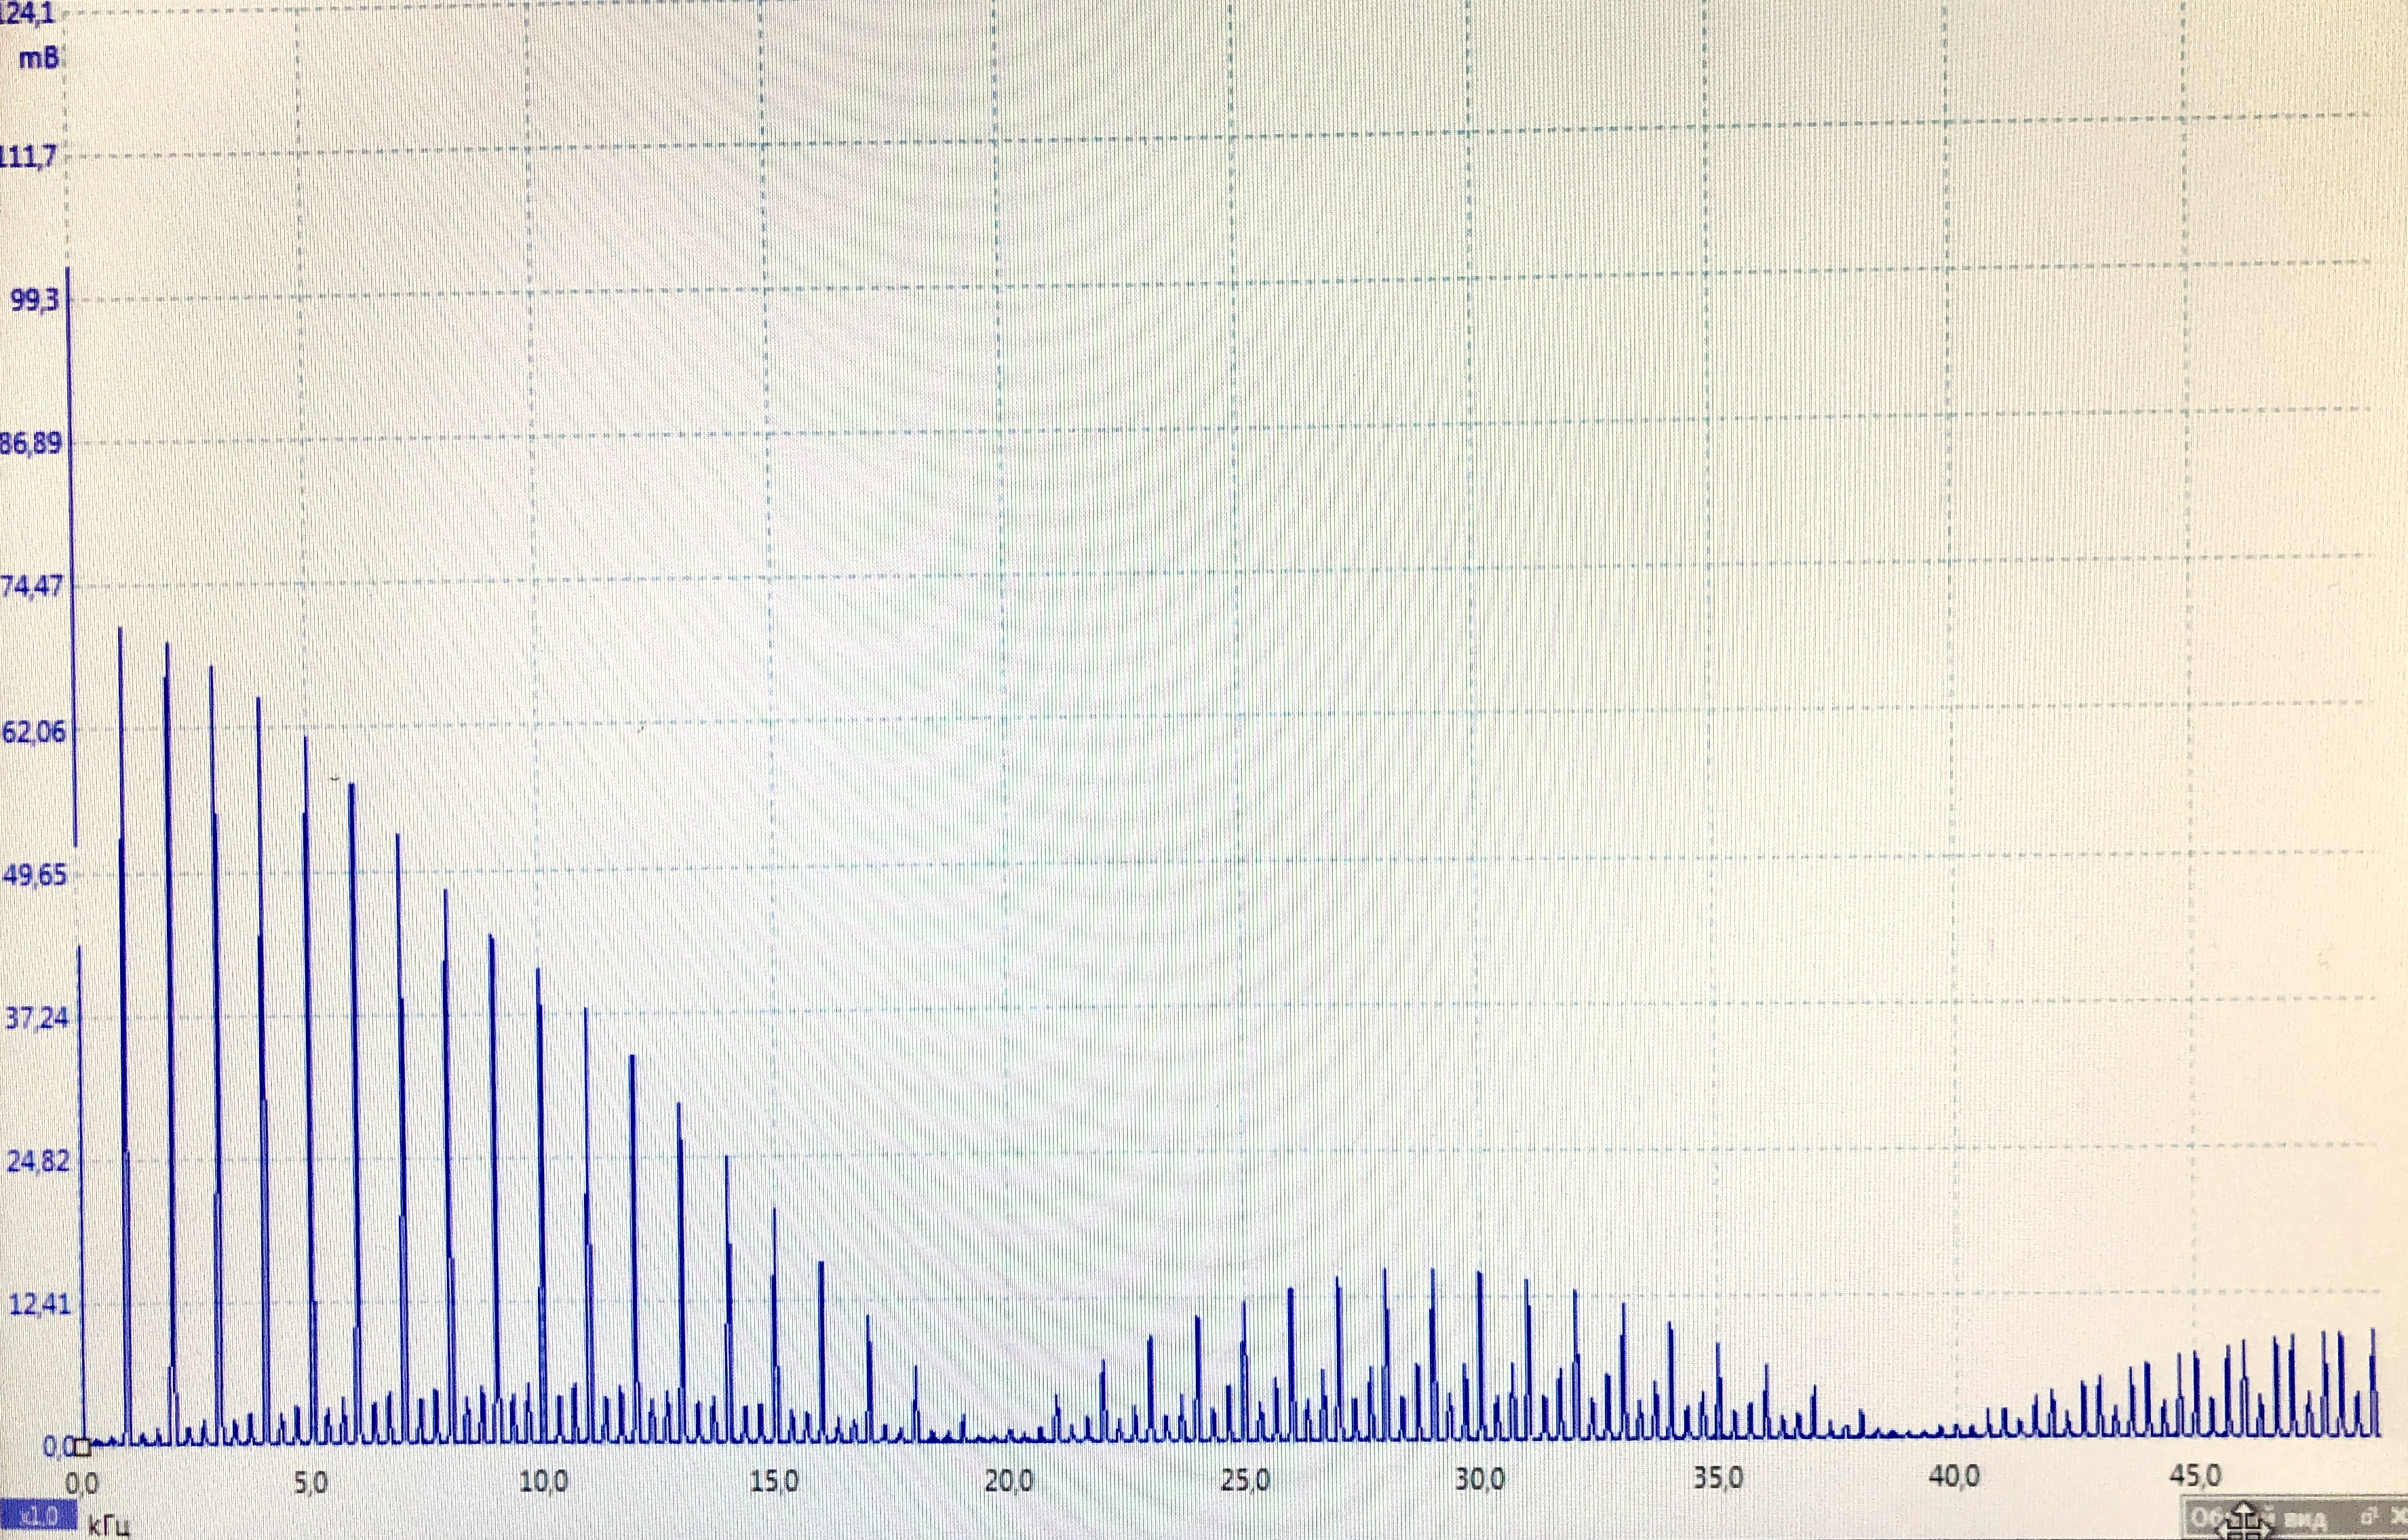
\includegraphics[width=0.6\linewidth]{1.jpeg}
    \caption[]{$\tau = 50мкс,\ f_{повт} = 1кГц$}
\end{figure}
\begin{figure}[h!]
    \centering
    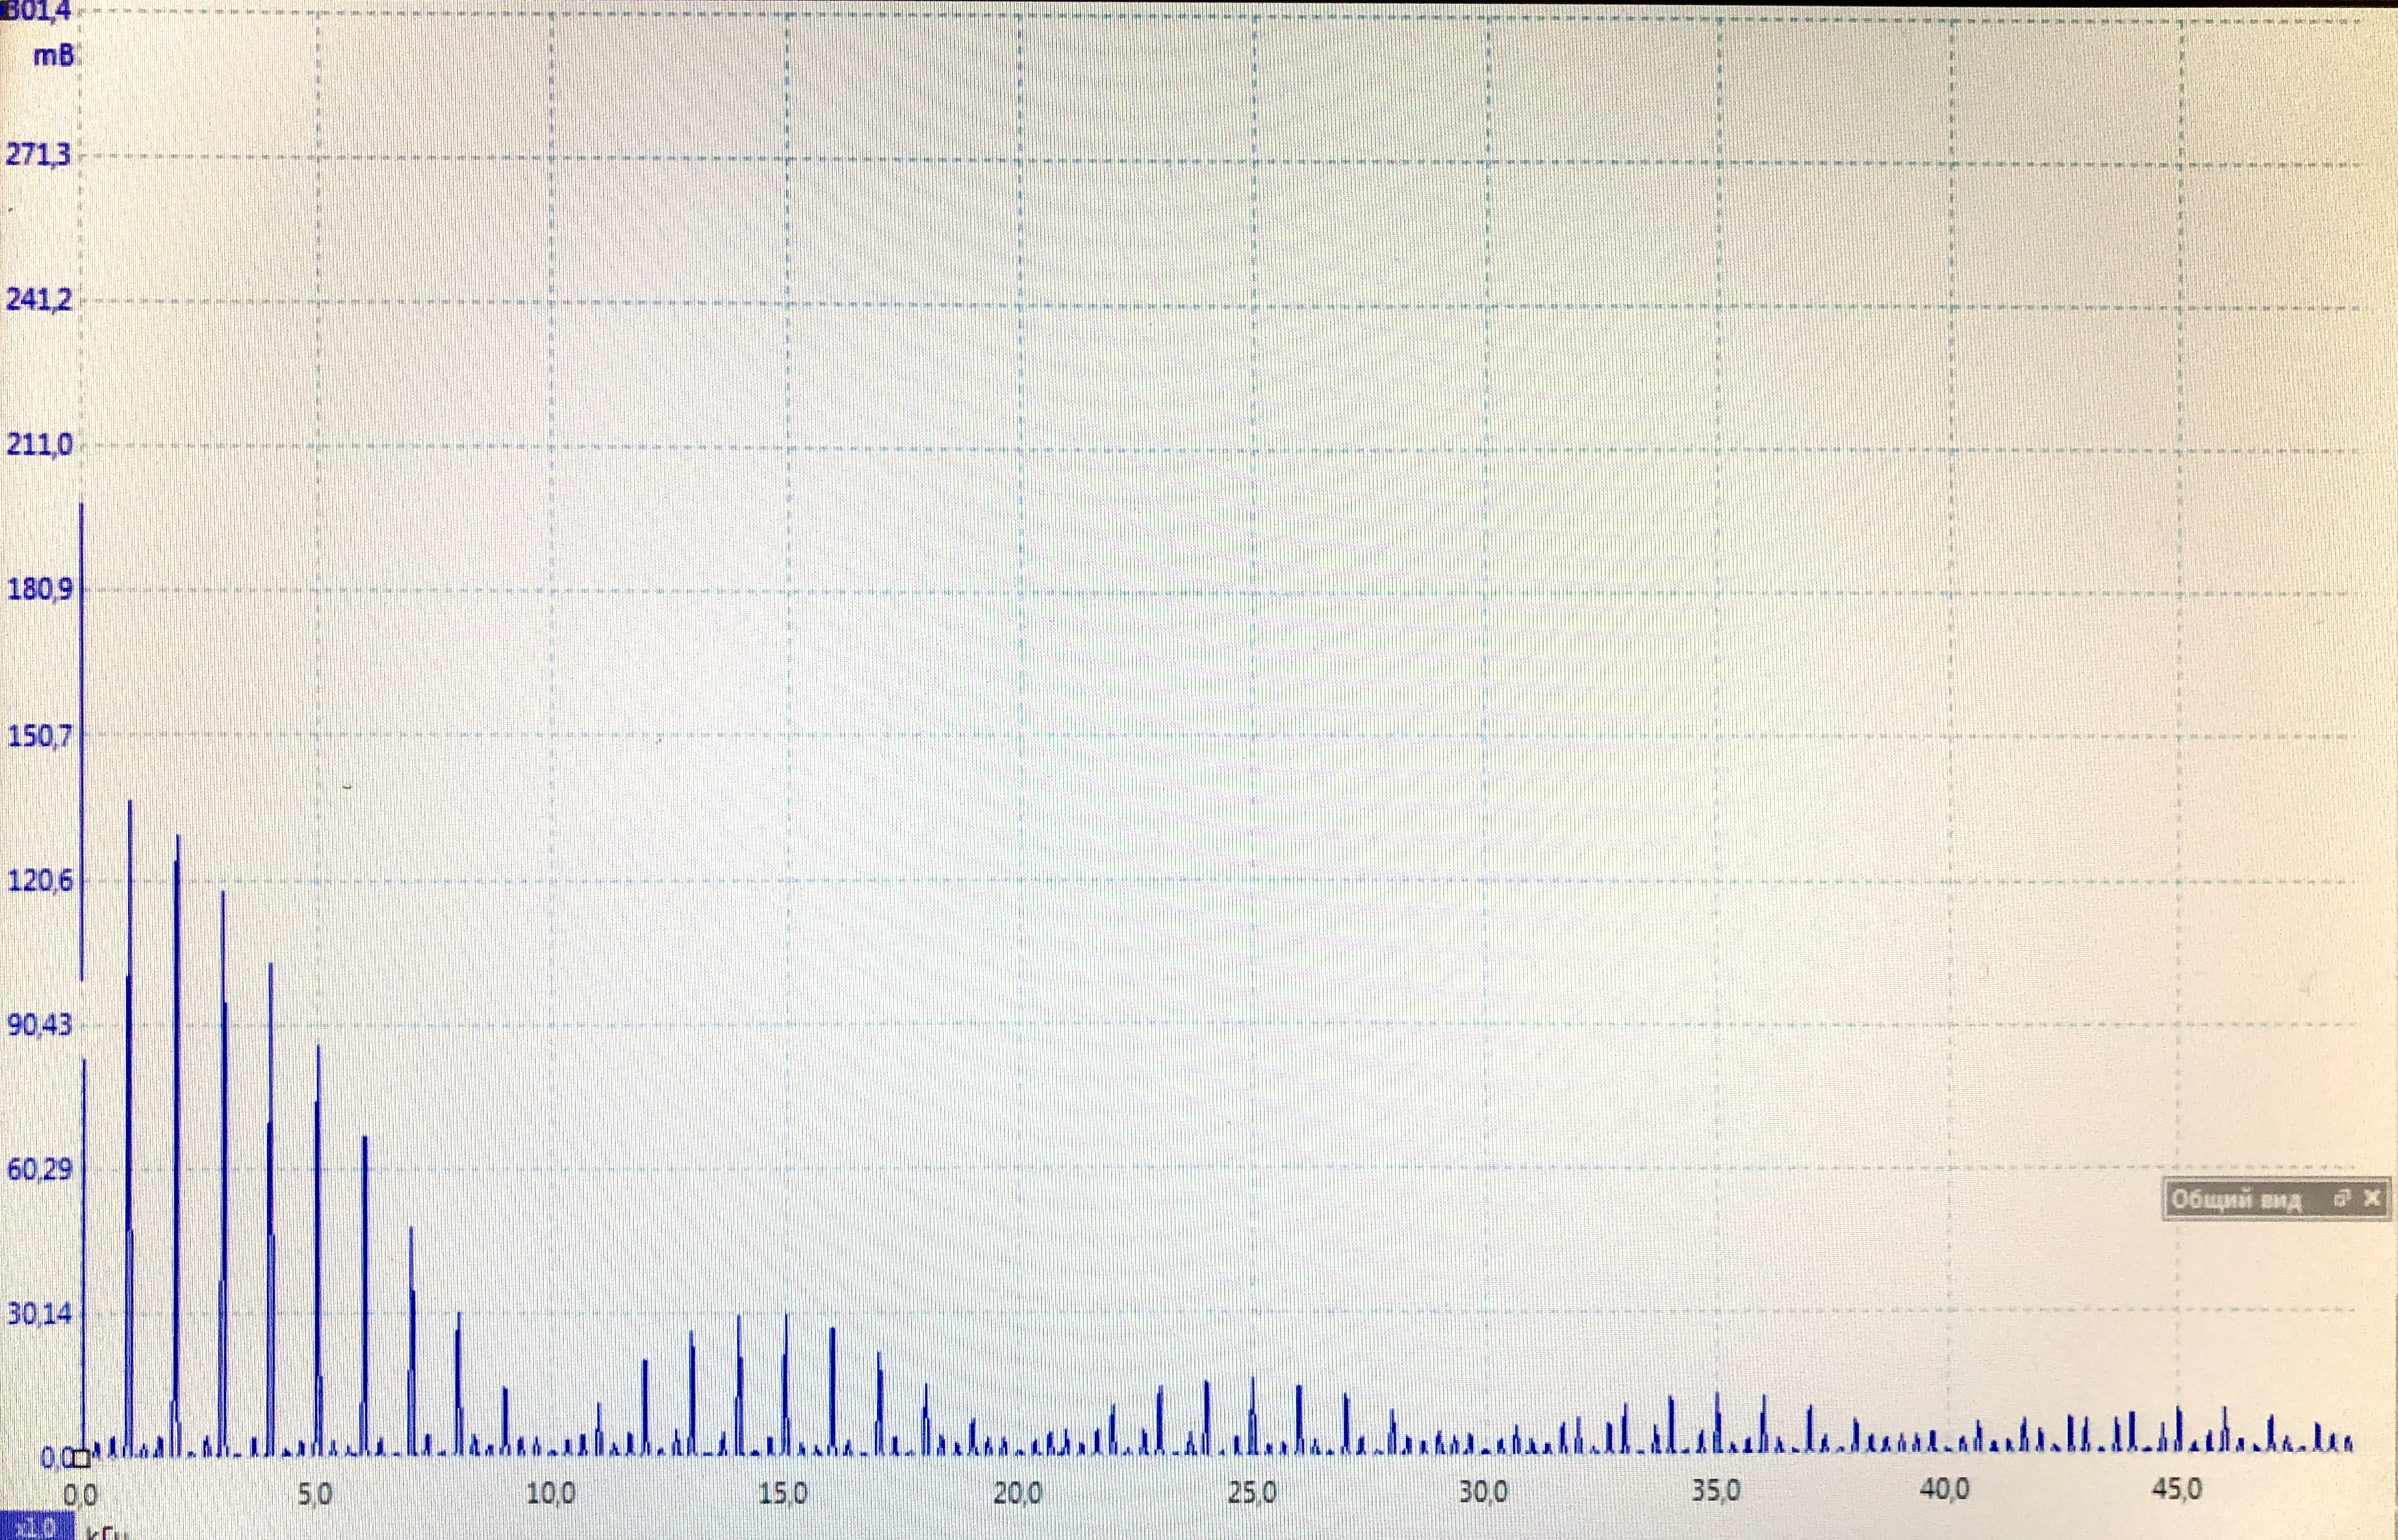
\includegraphics[width=0.5\linewidth]{2.jpeg}
    \caption[]{$\tau = 100мкс,\ f_{повт} = 1кГц$}
\end{figure}
\begin{figure}[h!]
    \centering
    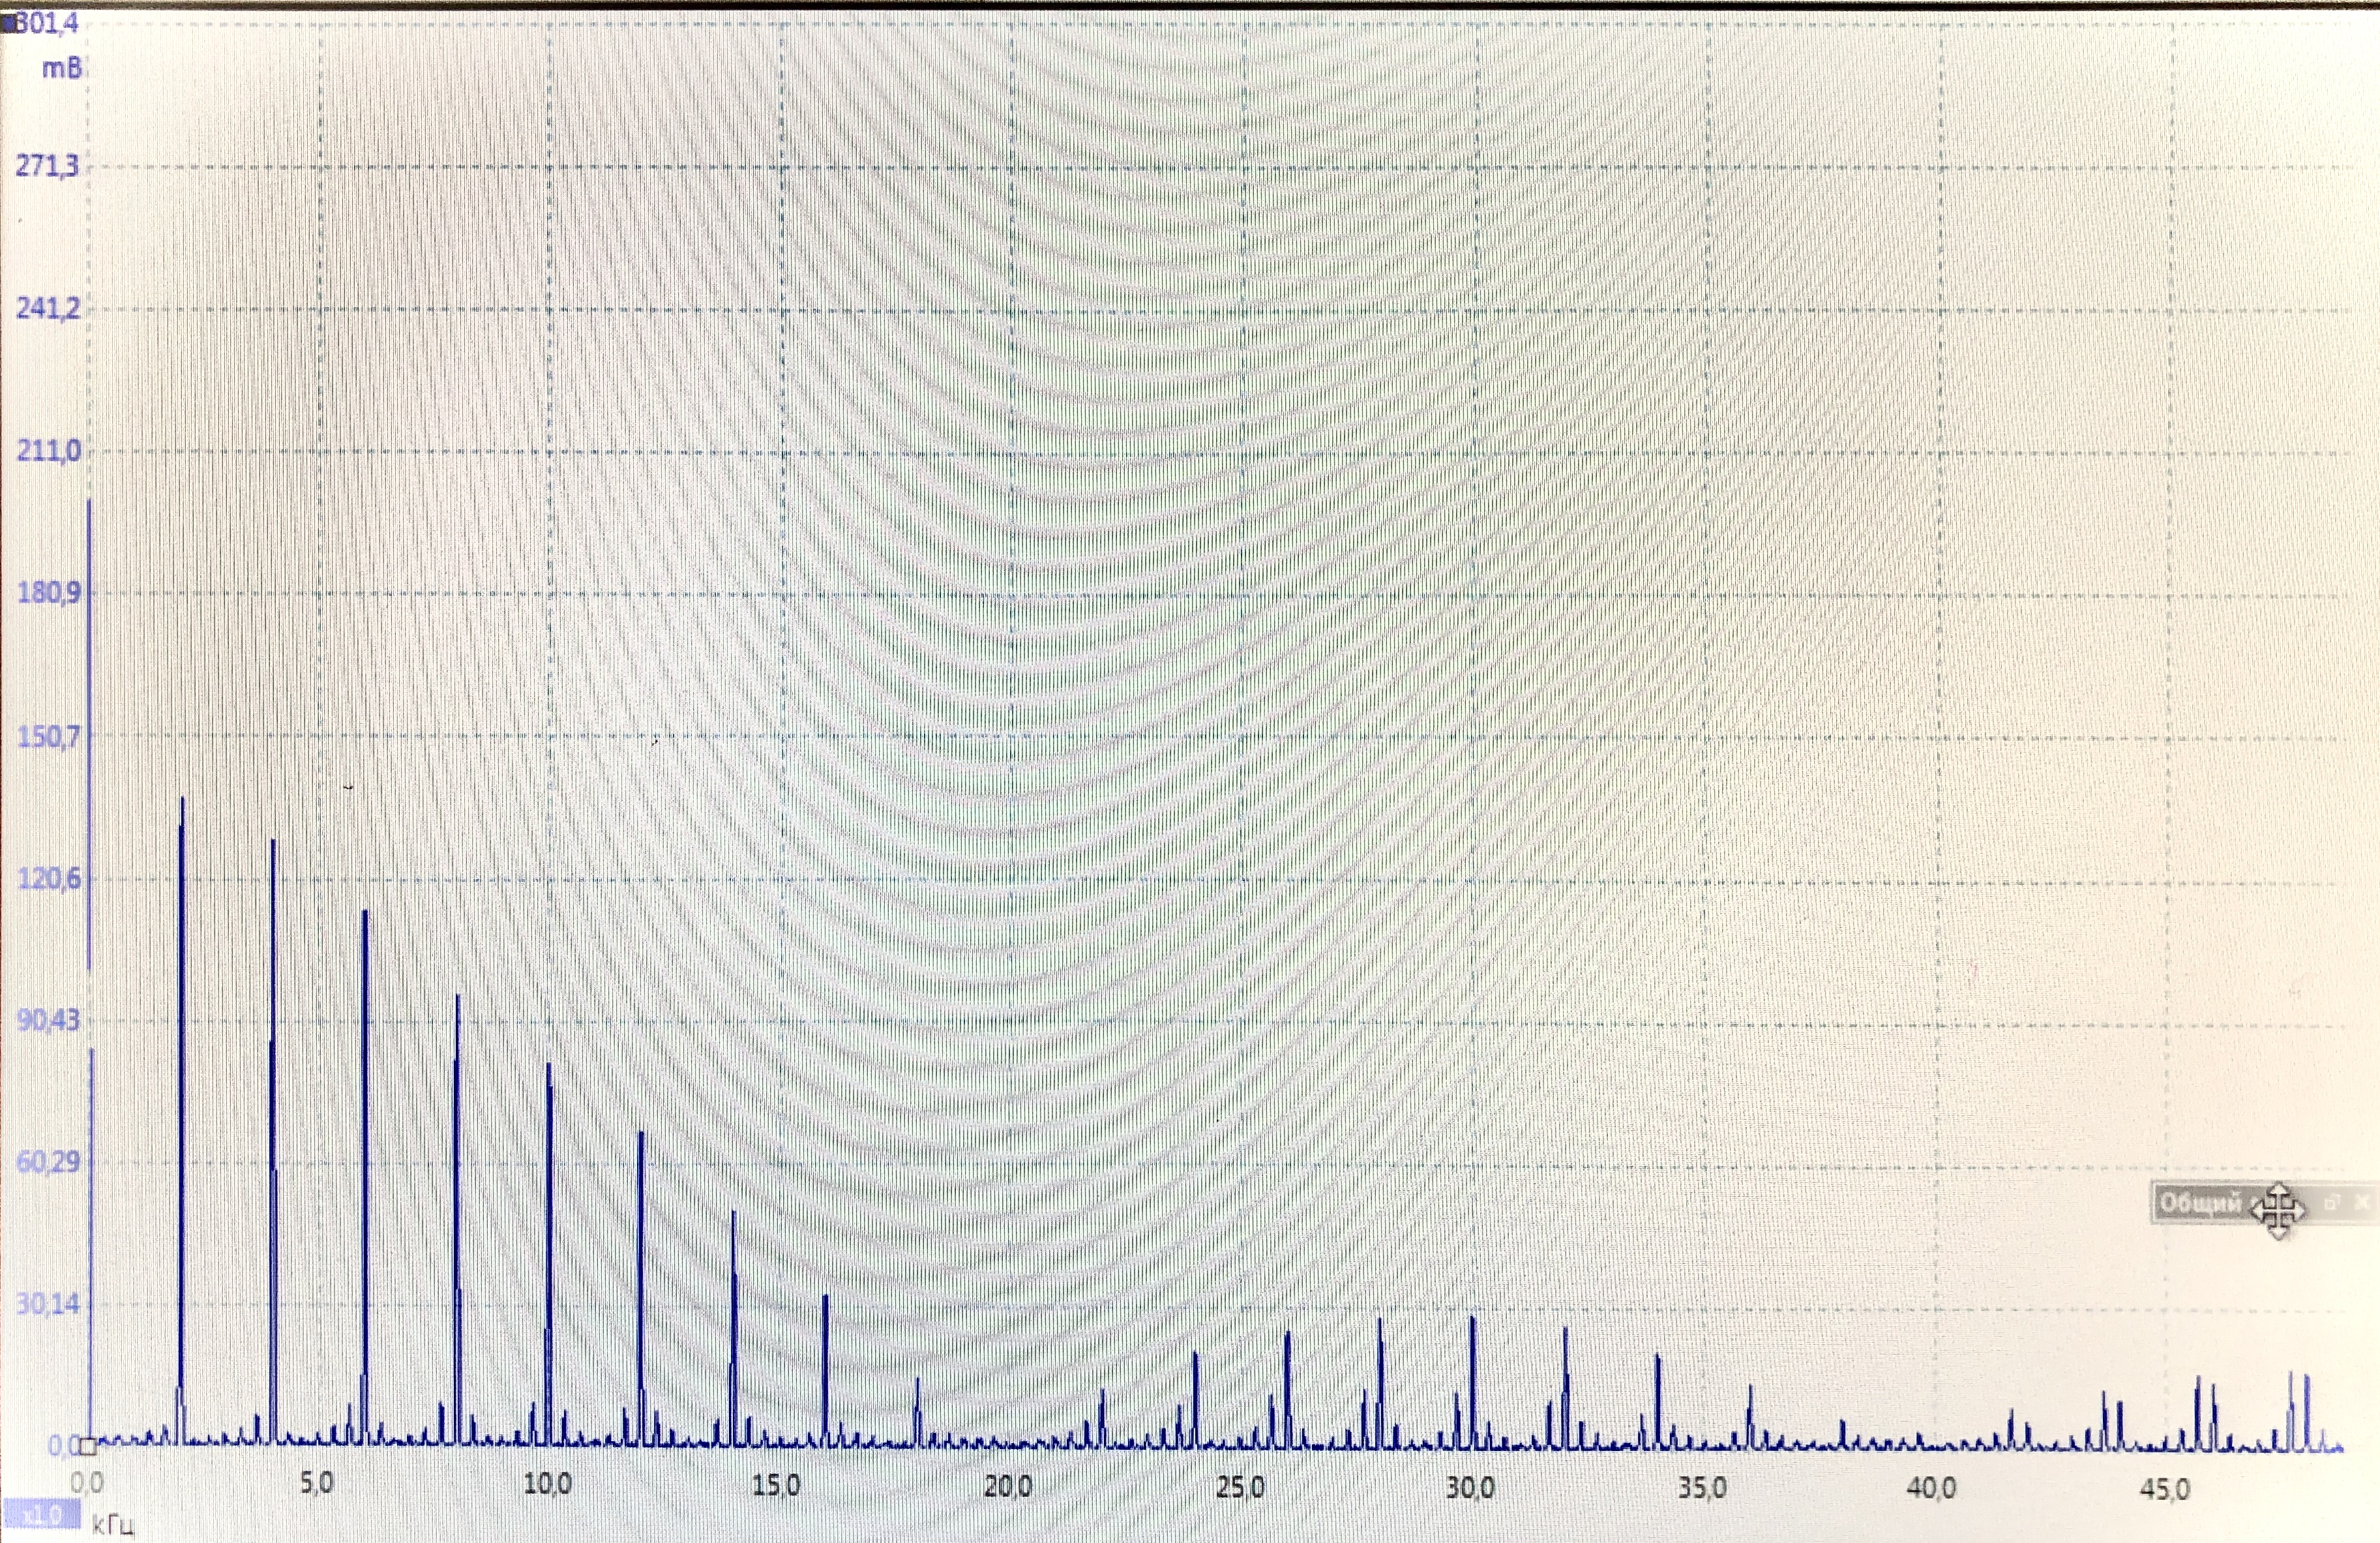
\includegraphics[width=0.5\linewidth]{3.jpeg}
    \caption[]{$\tau = 50мкс,\ f_{повт} = 2кГц$}
\end{figure}
\newpage
Теперь исследуем зависимость ширины спектра $\Delta\nu$ от $\tau$ при $f_{повт} = 1\ кГц$

\begin{table}[h!]
    \centering
    \begin{tabular}[]{|c|c|c|c|c|c|c|c|}
        \hline
        $\tau$, мкс & 25 & 50 & 75& 100& 125& 175& 200\\
        \hline
        $\Delta \nu$, кГц & 39.6 & 20.0 & 13.0 & 10.0 & 7.9& 5.5& 5.0\\
        \hline
        $1/\tau, \cdot 10^3\ с^{-1}$ & 40 & 20 & 13.3 & 10 & 8 & 5.7 & 5\\
        \hline
    \end{tabular}
    \caption{Исследование зависимости $\Delta \nu (\tau)$}
\end{table}

Проведем измерения частот и амплитуд у различных гармоник сигналов с различной длительностью импульсов
\begin{table}[h!]
    \centering
    $\tau = 50$мкс, $f_{повт} = 1$кГц

    \begin{tabular}[]{|c|c|c|c|c|c|c|c|c|}
        \hline
        n & 1&2&3&4&5&6&7&8\\
        \hline
        $\nu$, кГц & 0.004&1.000&2.003&3.005&4.006&4.993&5.996&6.997\\
        \hline
        A, мВ&15.66&3.165&3.022&2.815&2.625&2.522&2.514&2.450\\
        \hline
    \end{tabular}
\end{table}

\begin{table}[h!]
    \centering
    $\tau = 100$мкс, $f_{повт} = 1$кГц

    \begin{tabular}[]{|c|c|c|c|c|c|c|c|c|}
        \hline
        n & 1& 2& 3& 4& 5 & 6& 7& 8\\
        \hline
        $\nu$, кГц &  0.001& 1.003& 2.001& 3.005& 4.005& 4.996& 5.994& 6.998\\
        \hline
        A, мВ& 2.041& 6.139& 5.677& 5.018& 4.224 & 3.604& 2.955 &2.224\\
        \hline
    \end{tabular}
\end{table}

На рис. 5 изображен график, построенный по полученным значениям.
По МНК получаем, что $k\approx 0.99 \pm 0.01$, что подтверждает теоретические расчеты.

\begin{figure}[h!]
    \centering
    \includegraphics[width=0.7\linewidth]{dv(1_t).png}
    \caption{Зависимость $\Delta \nu (1/\tau)$}
\end{figure}


\subsection{Исследование спектра периодической последовательности цугов гармонических колебаний}

    При увеличении длительности импульса вдвое произошли изменения, аналогичные с первой частью работы.
    Изображения представлены на рис. 6 и рис. 7
\begin{figure}[h!]
    \centering
    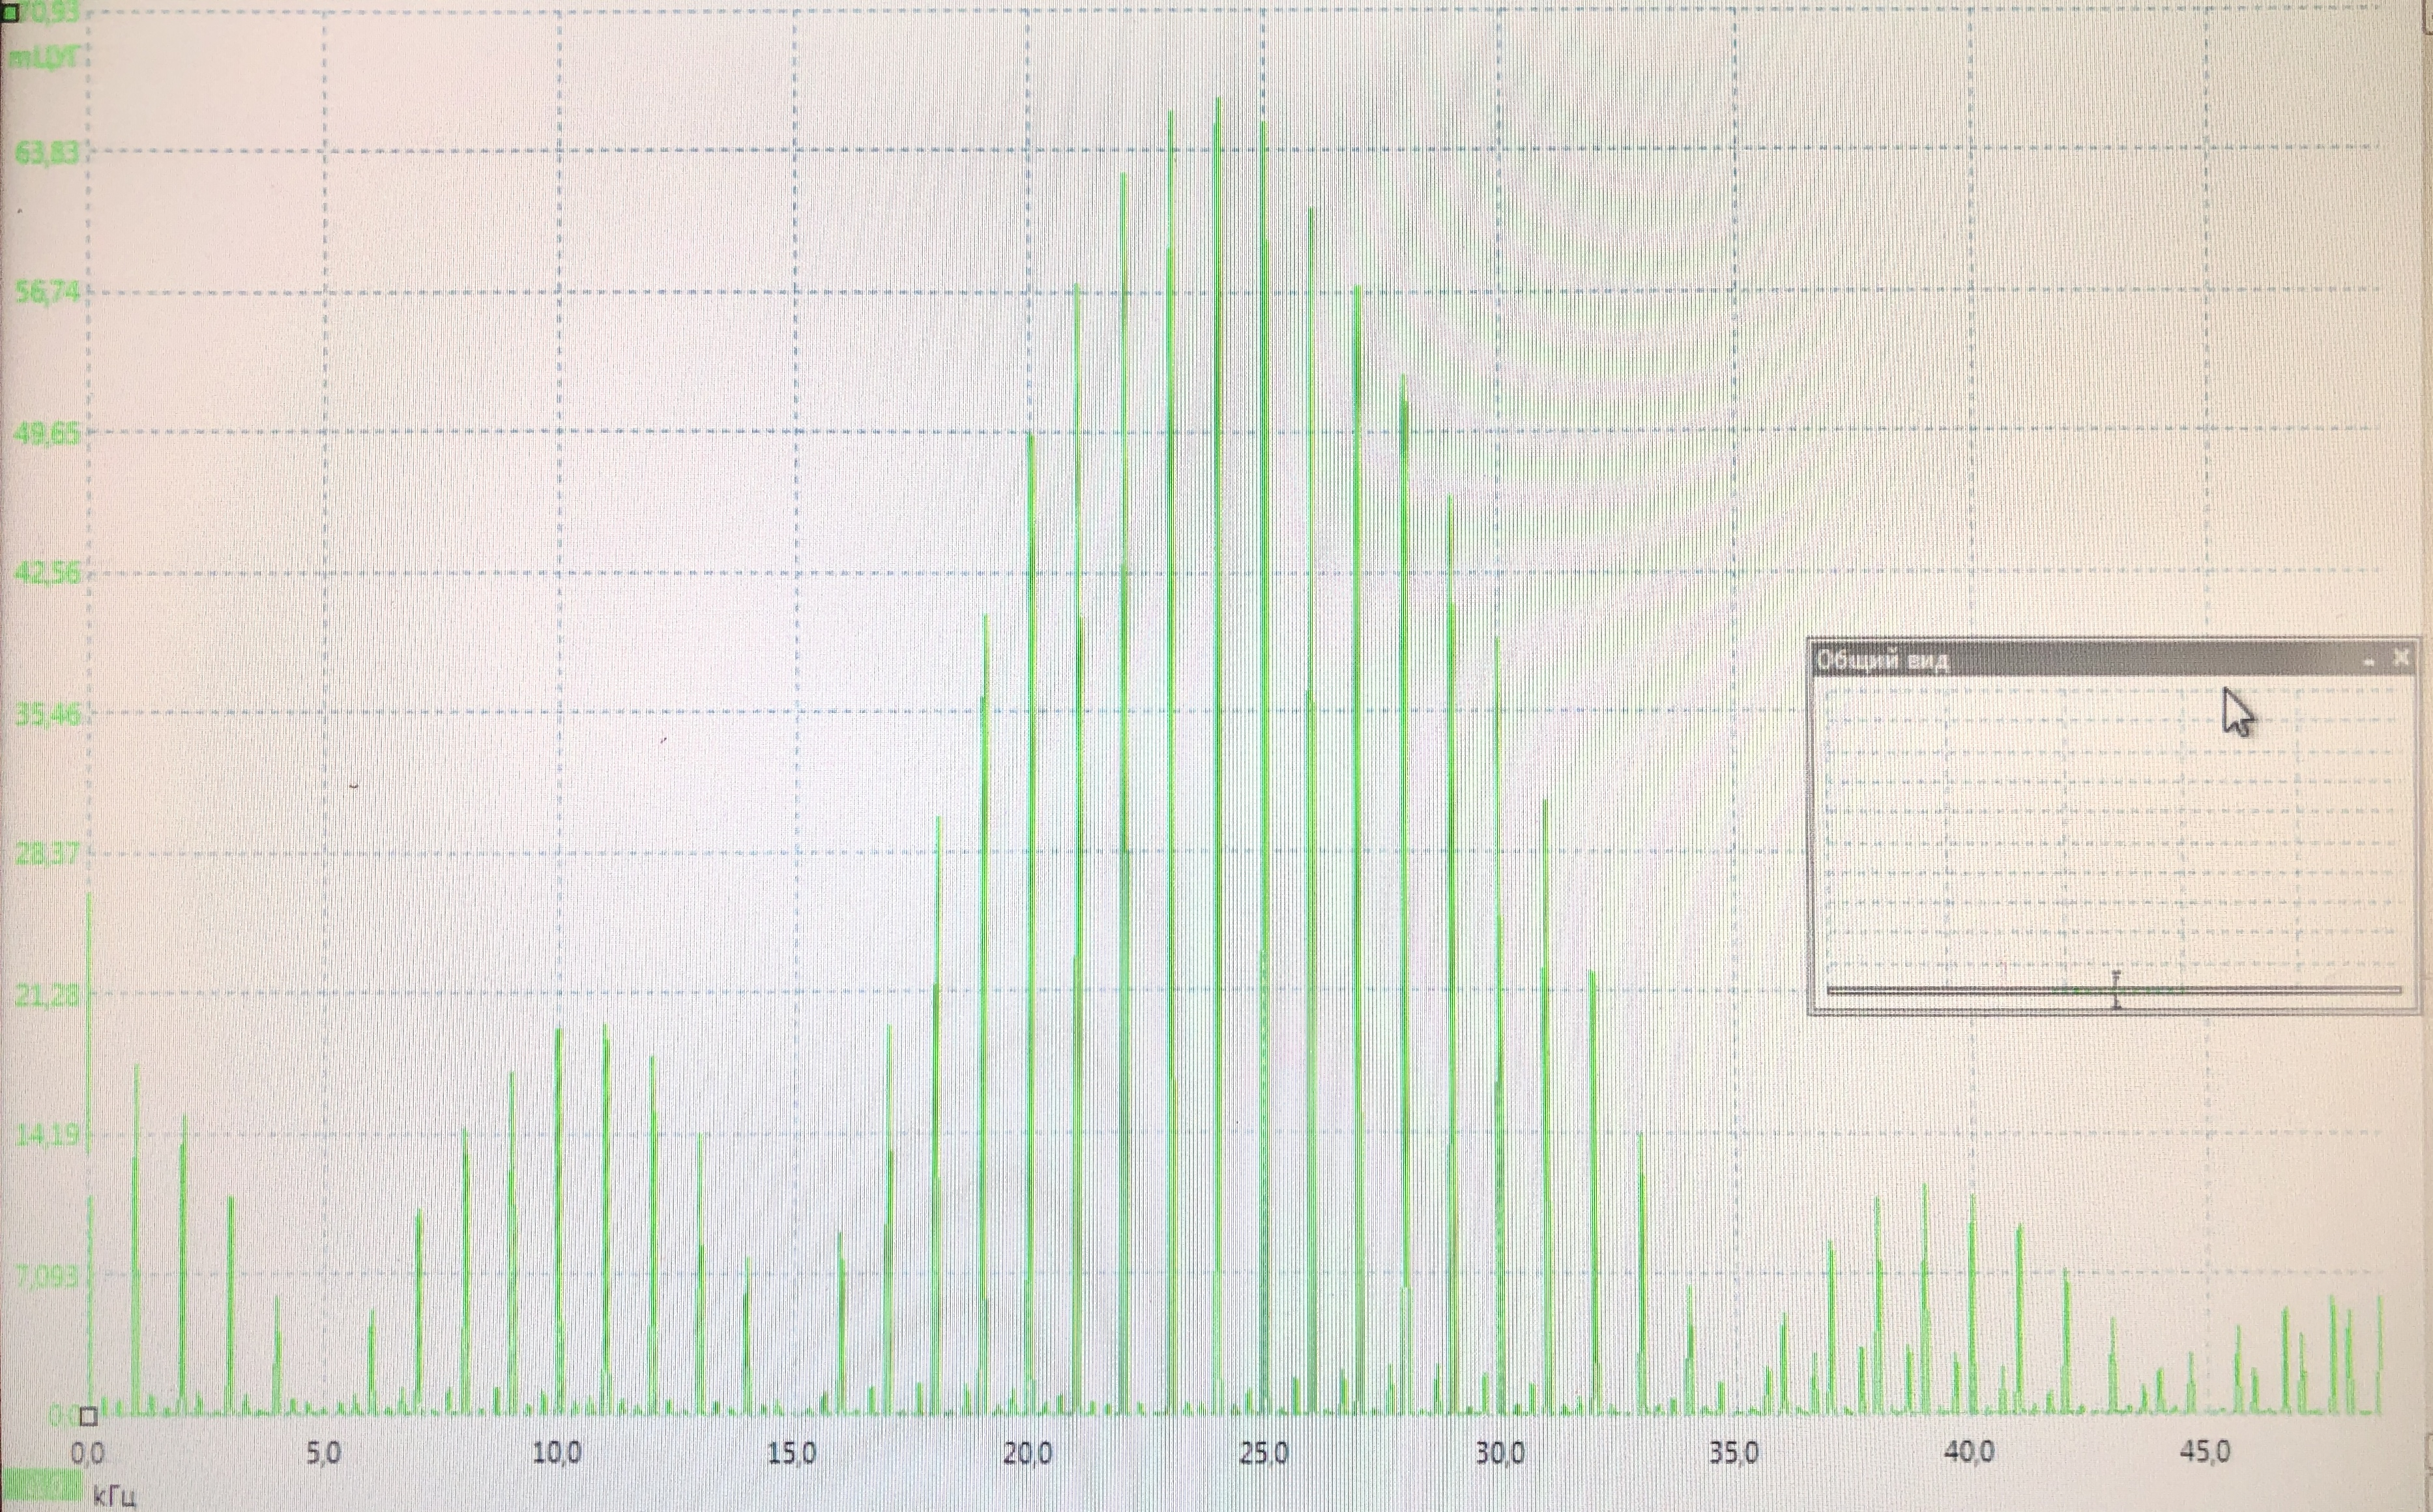
\includegraphics[width=0.5\linewidth]{4.jpeg}
    \caption[]{$\tau = 50мкс,\ f_{повт} = 1кГц$}
\end{figure}
\begin{figure}[h!]
\centering
    \includegraphics[width=0.5\linewidth]{5.jpeg}
    \caption[]{$\tau = 100мкс,\ f_{повт} = 1кГц$}
\end{figure}
\newpage

    При изменении $f_{повт}$ (10, 25 и 40 кГц) изображение меняло свое положение по горизонтальной оси (рис. 7, 8, 9).

\begin{figure}[h!]
    \centering
    \includegraphics[width=0.6\linewidth]{7.jpeg}
    \caption[]{$f_{повт} = 10$ кГц}
    \end{figure}
\begin{figure}[h!]
\centering
    \includegraphics[width=0.6\linewidth]{6.jpeg}
    \caption[]{$f_{повт} = 25$ кГц}
    \end{figure}
\begin{figure}[h!]
\centering
    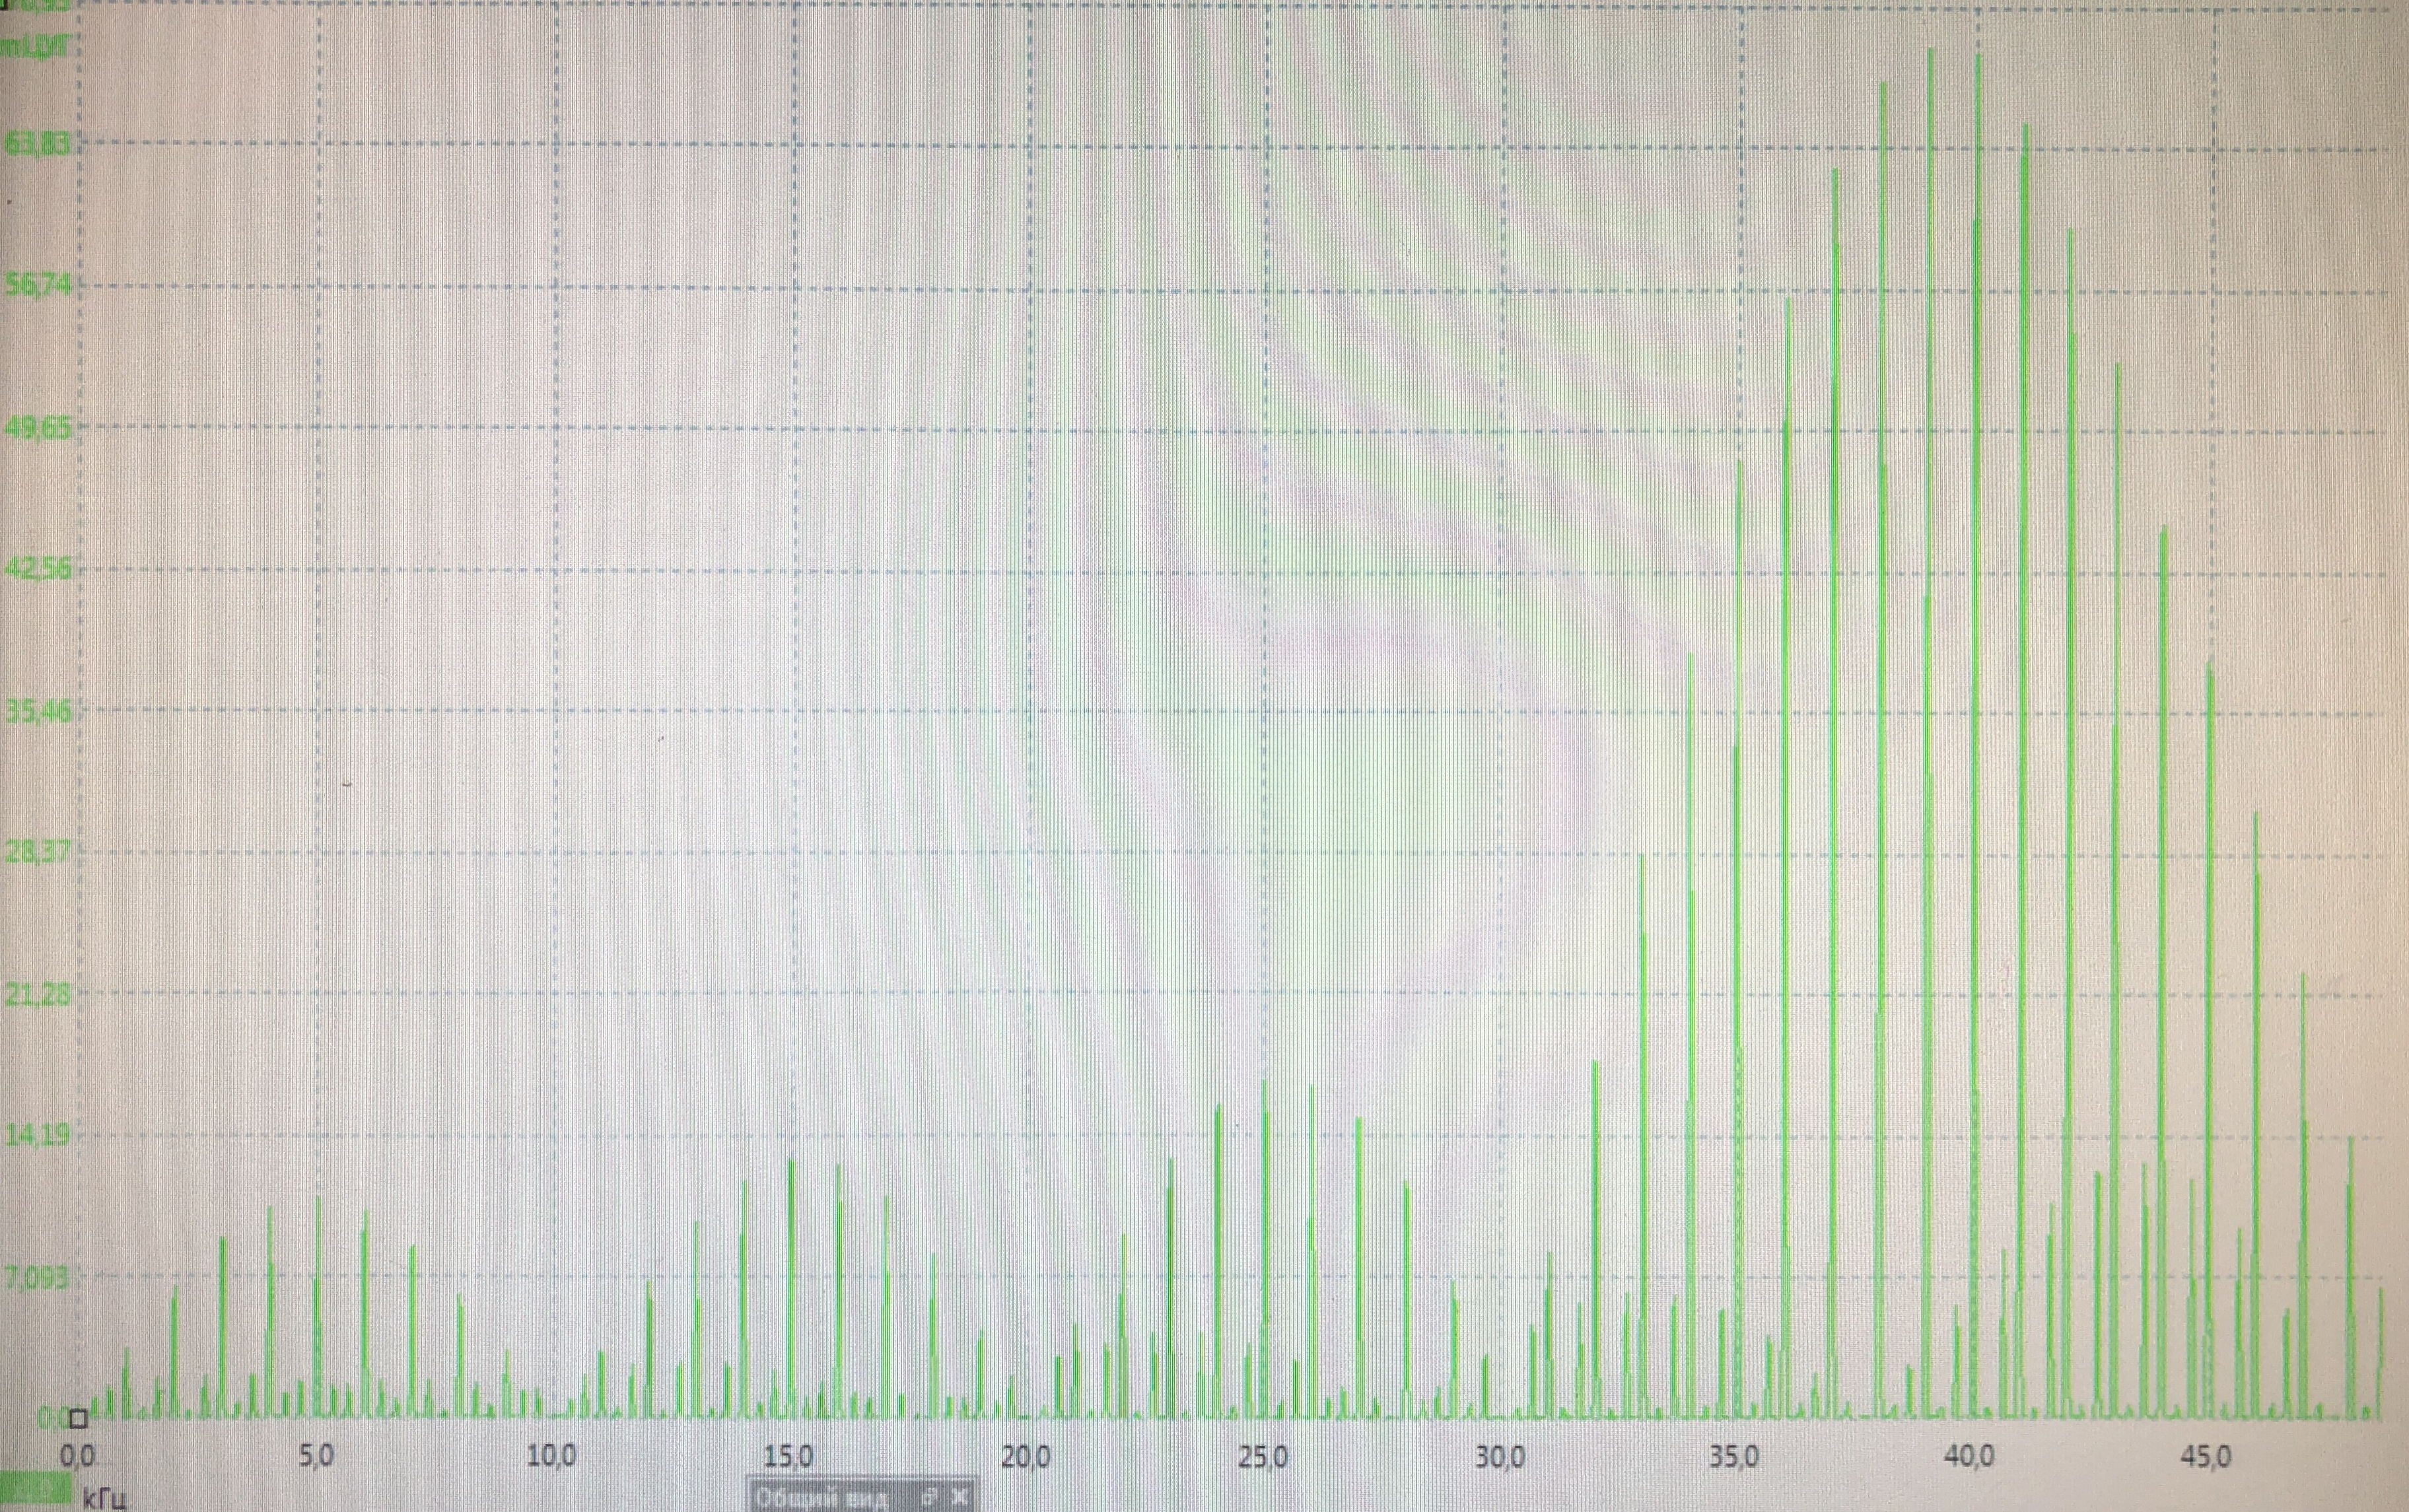
\includegraphics[width=0.5\linewidth]{8.jpeg}
    \caption[]{$f_{повт} = 40$ кГц}
\end{figure}

    Теперь установим значения $\nu_0 = 30$ кГц, $\tau = 100$ мкс и проведем измерение зависимости $\delta \nu$ от $f_{повт}$
  \begin{table}[h!]
    \newline
    \centering
    \begin{tabular}[]{|c|c|c|c|c|c|}
        \hline
        $f_{повт}$, кГц & 0.5& 1& 2& 4& 5\\
        \hline
        $\delta \nu$, кГц & 0.5& 1& 2&4 & 5\\
        \hline
    \end{tabular}
    \caption{Исследование зависимости $\delta \nu(f_{повт})$}
\end{table}

    Измерим частоты и амплитуды различных гармоник при $f_{повт}$ = 100 и 200 кГц
    \newline
\begin{table}[h!]
    \
    $f_{повт}$ = 1 кГц, $\tau = 100$ мкс 

    \begin{tabular}[]{|c|c|c|c|c|c|c|c|c|}
        \hline
        n &  1& 2& 3& 4& 5 & 6& 7 & 8 \\
        \hline
        $\nu$, кГц &  30.02 & 31.00& 31.95& 33.00&33.98 & 34.96 &36.02&36.92\\
        \hline
        A, мкВ& 12.160& 7.962& 7.452 & 6.601 & 5.678& 4.415& 3.347& 2.496 \\
        \hline
    \end{tabular}
    \newline

    $f_{повт}$ = 2 кГц, $\tau = 100$ мкс 

    \begin{tabular}[]{|c|c|c|c|c|c|c|c|c|c|c|c|}
        \hline
        n & 1& 2& 3& 4& 5 & 6& 7 & 8 \\
        \hline
        $\nu$, кГц &  30.04 & 31.08& 32.11& 33.45&34.00 & 35.08 &36.66&37.03\\
        \hline
        A, мкВ& 25.008& 15.098& 14.908 & 13.201 & 11.098& 9.802& 6.701& 5.007 \\
        \hline
    \end{tabular}
\end{table}

    Построим график по полученным значениям (рис. 11). 
    Здесь коэффициент наклона также равен 1, что соответсвует расчетам.
    \begin{figure}[h!]
    \centering
    \includegraphics[width=0.4\linewidth]{f(v).png}
    \caption{Зависимость $\delta\nu (f_{повт})$}
\end{figure}

\newpage 

\subsection{Исследование спектра гармонических сигналов, модулированных по амплитуде}
Установим $\nu_0 = 25$ кГц и $f_{mod} = 1$ кГц.

Обозначим ${A_{max} - A_{min} \over A_{max} + A_{min}} = m,\ {A_{бок} \over A_{осн}} = k$ и снимем зависимость $k(m)$
\begin{table}[h!]
    \centering
    \begin{tabular}[]{|c|c|c|c|c|c|}
        \hline
        A, мВ & 2& 0.8& 1.2& 1.6& 0.4\\
        \hline
        $A_{max}$, мЦУГ & 990& 707& 790& 890& 601 \\
        \hline
        $A_{min}$, мЦУГ & 17& 293& 200& 103& 398\\
        \hline
        $A_{осн}$, мЦУГ &317.5  &321 & 322& 322& 321\\
        \hline
        $A_{бок}$, мЦУГ & 163.5& 63.5& 96& 125& 31 \\
        \hline
        $m$ & 6.3 & 1.6 & 2.6 & 4.0 & 0.7 \\
        \hline
        $k$ & 0.5 & 0.2 & 0.3 & 0.4 & 0.1 \\
        \hline
    \end{tabular}
    \caption{Исследование зависимости $k(m)$}
\end{table}

\begin{figure}[h!]
    \centering
    \includegraphics[width=0.7\linewidth]{k(m).png}
    \caption{Исследование зависимости $k(m)$}
\end{figure}

Полученное значение углового наклона $k' = 0.51 \pm 0.01$, что сходится с теоретическим значением. 
\section{Подведение итогов}
В ходе работы был изучен спектральный состав периодических электрических сигналов различных форм: прямоугольные импульсы, цуги гармонических колебаний и сигналы, модулированные по амплитуде. 
Полученные результаты подтверждают установленные соотношения.
\end{document}